% CSUF MPA Orientation — Fall 2026
% Author: David Adams

\documentclass[10pt,aspectratio=169]{beamer}
% Handout mode toggle
\newif\ifhandout
\ifhandout
  \usepackage{pgfpages}
  \pgfpagesuselayout{4 on 1}[letterpaper, landscape]
\fi

\usetheme{CSUFTitan}

% --------------------
% Title metadata
% --------------------
\title{Master of Public Administration Program}
\subtitle{MPA Student Orientation}
\date{Fall 2026}
\CSUFSetTitleGraphic{images/PUBLIC-ADMINISTRATION-color2.png}
\CSUFSetFooterLogos[0.34cm]
  {images/CalStateFullerton-color-R.png}
  {images/CalStateFullerton-reversed-R.png}

% --------------------
\begin{document}
% --------------------

\maketitle

\section{\textcolor{titanorange}{Welcome}}
\begin{frame}{Welcome}
\begin{Large}
  \textbf{We are glad you are here.}\par\vspace{0.5em}
  Today is about meeting each other, getting oriented, and helping you feel confident about the program.\par\vspace{0.75em}

  \textbf{Land Acknowledgment}\par
  We gather on the ancestral lands of the Tongva and Acjachemen peoples. We honor their past, present, and future stewardship, and we commit to learning and working with respect for this place.
\end{Large}
\end{frame}

\begin{frame}{Agenda}
\footnotesize
\begin{columns}[T,totalwidth=\textwidth]
  \begin{column}{0.33\textwidth}
    \textbf{Large Group}
    \begin{itemize}\setlength{\itemsep}{0pt}
      \item Welcome and Introductions
      \item Why CSUF?
      \item Mission, Vision, Values
      \item Public Administration Student Association (PASA)
    \end{itemize}
  \end{column}

  \begin{column}{0.33\textwidth}
    \textbf{Breakouts}
    \begin{enumerate}\setlength{\itemsep}{0pt}
      \item \textbf{New Students}
        \begin{itemize}\setlength{\itemsep}{0pt}
          \item Faculty Profiles
          \item Curriculum
          \item Milestones
          \item Scholarships and Awards
        \end{itemize}
      \item \textbf{Family/Friends,Current Students, Alums}
        \begin{itemize}\setlength{\itemsep}{0pt}
          \item Supporting your MPA Student
          \item Navigating Grad School
          \item Success Strategies
        \end{itemize}
    \end{enumerate}
  \end{column}

  \begin{column}{0.33\textwidth}
    \textbf{Large Group}
    \begin{itemize}\setlength{\itemsep}{0pt}
      \item Success and Support
      \item Campus Resources
      \item Contact Information
      \item Large Group Q\&A
    \end{itemize}
  \end{column}
\end{columns}
\end{frame}

\begin{frame}{Introductions}
\begin{columns}[c,onlytextwidth]
  \column{0.34\textwidth}
    \centering
    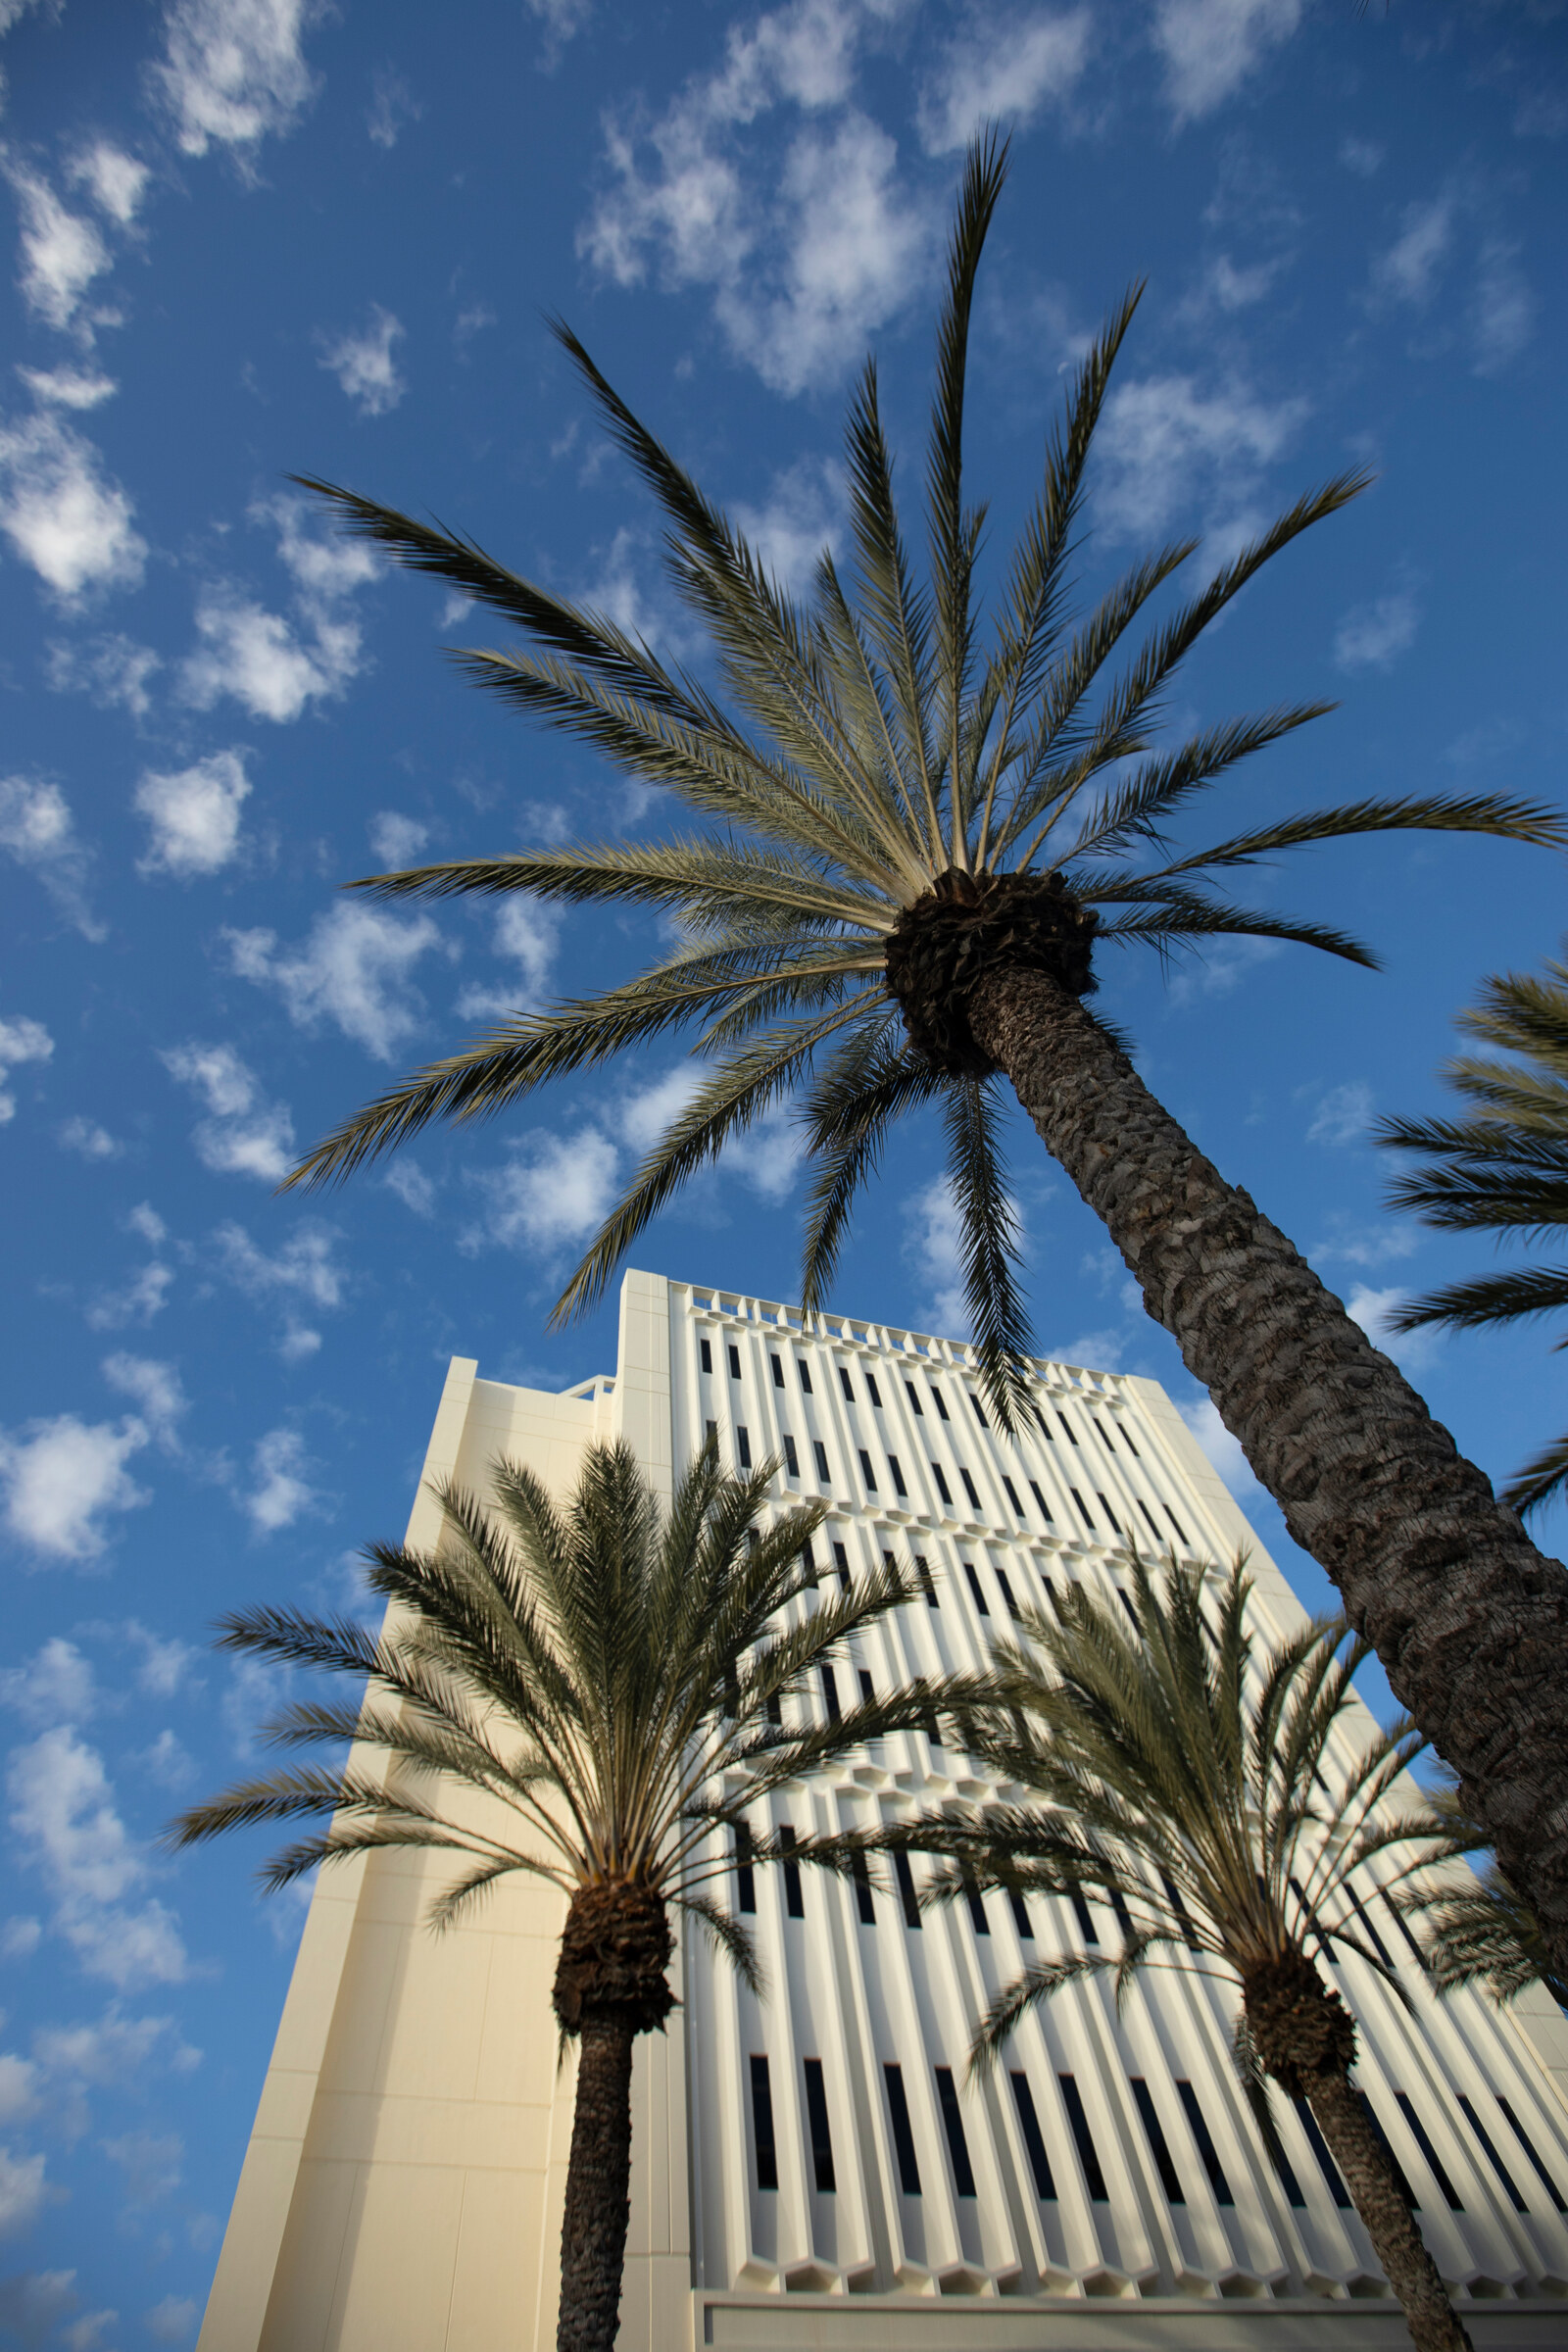
\includegraphics[height=5.25cm,keepaspectratio]{images/campus_palm_tower.jpg}

  \column{0.61\textwidth}
    {\large\textbf{Let's meet the MPA community.}}
    \begin{Large}
    \begin{itemize}\setlength{\itemsep}{9pt}
      \item Faculty
      \item Incoming MPA students
      \item Current MPA students
      \item Alums
    \end{itemize}
    \end{Large}
    \small
    Please share your name, your role or program status, and what brought you to the MPA.
\end{columns}
\end{frame}

\section{\textcolor{titanorange}{Why CSUF}}
\begin{frame}{Program by the Numbers}
\begin{Large}
\begin{itemize}
  \item \textbf{1968:} Serving Orange County since 1968
  \item \textbf{\(\sim\)93:} Students; cohorts begin year-round
  \item \textbf{\(\sim\)30:} Graduates each year
  \item \textbf{4:} Concentrations offered
  \item \textbf{2--3 years:} Typical full-time/part-time completion
\end{itemize}
\end{Large}
\end{frame}

\begin{frame}{The Value of a CSUF MPA}
\begin{Large}
\begin{itemize}
  \item \textbf{Evening courses} designed for working professionals
  \item \textbf{Flexible formats:} in-person, synchronous online, and hybrid
  \item \textbf{Strong regional network} across public and nonprofit agencies
  \item \textbf{NASPAA accredited} since 1989
\end{itemize}
\end{Large}
\end{frame}

\section{\textcolor{titanorange}{Mission, Vision, and Values}}

\begin{frame}{Our Mission and Vision}
\textbf{Mission}\\
We prepare leaders to address complex social issues, uphold democratic values, and foster ethical, equitable, and inclusive public service in Orange County and beyond.

\vspace{0.8em}
\textbf{Vision}\\
To be recognized for excellence in value-driven public service and community engagement.
\end{frame}

\begin{frame}{Our Values}
\begin{columns}[T,onlytextwidth]
  \column{0.485\textwidth}
    \begin{block}{Accountability}
      Be transparent, responsive, and evidence-informed to sustain public trust.
    \end{block}

  \column{0.485\textwidth}
    \begin{block}{Ethics}
      Practice integrity and fairness, with service to the public good at the center of decisions.
    \end{block}
\end{columns}

\vspace{0.35em}
\begin{columns}[T,onlytextwidth]
  \column{0.485\textwidth}
    \begin{block}{Collaboration}
      Build inclusive partnerships across agencies, sectors, and communities.
    \end{block}

  \column{0.485\textwidth}
    \begin{block}{Lifelong Learning}
      Keep learning, reflecting, and adapting throughout a career in public service.
    \end{block}
\end{columns}
\end{frame}

\section{\textcolor{titanorange}{Public Administration Student Association (PASA)}}

\begin{frame}{Public Administration Student Association (PASA)}
  \centering
  
\includegraphics[width=\textwidth,height=5.2cm,keepaspectratio]{images/join_PASA.png}
\end{frame}

\section{\textcolor{titanorange}{Breakout Groups}}

\begin{frame}{Breakout Groups}
\begin{columns}[T,onlytextwidth]
  \column{0.45\textwidth}
  \textbf{Breakout Group 1: New Students}
  \begin{itemize}
    \item Program structure
    \item Concentrations
    \item Milestones
  \end{itemize}

  \column{0.55\textwidth}
  \textbf{Breakout Group 2: Family, Alums, Current Students}
  \begin{itemize}
    \item Supporting your MPA Student
    \item Understanding the program
    \item Navigating Grad School
    \item Success Strategies
  \end{itemize}
\end{columns}
\end{frame}

\begin{frame}{Your Public Service Starting Point}
\begin{columns}[c,onlytextwidth]
  \column{0.64\textwidth}
    {\large\textbf{Let's go around the room.}}
    \begin{Large}
    \begin{enumerate}\setlength{\itemsep}{7pt}
      \item Your name
      \item Your current role or area of interest
      \item One public issue you hope to help solve
    \end{enumerate}
    \end{Large}
    \vspace{0.4em}
    \alert{\textbf{Aim for about 20 seconds.}}\\
    \small We are putting names, interests, and faces together.

  \column{0.31\textwidth}
    \centering
    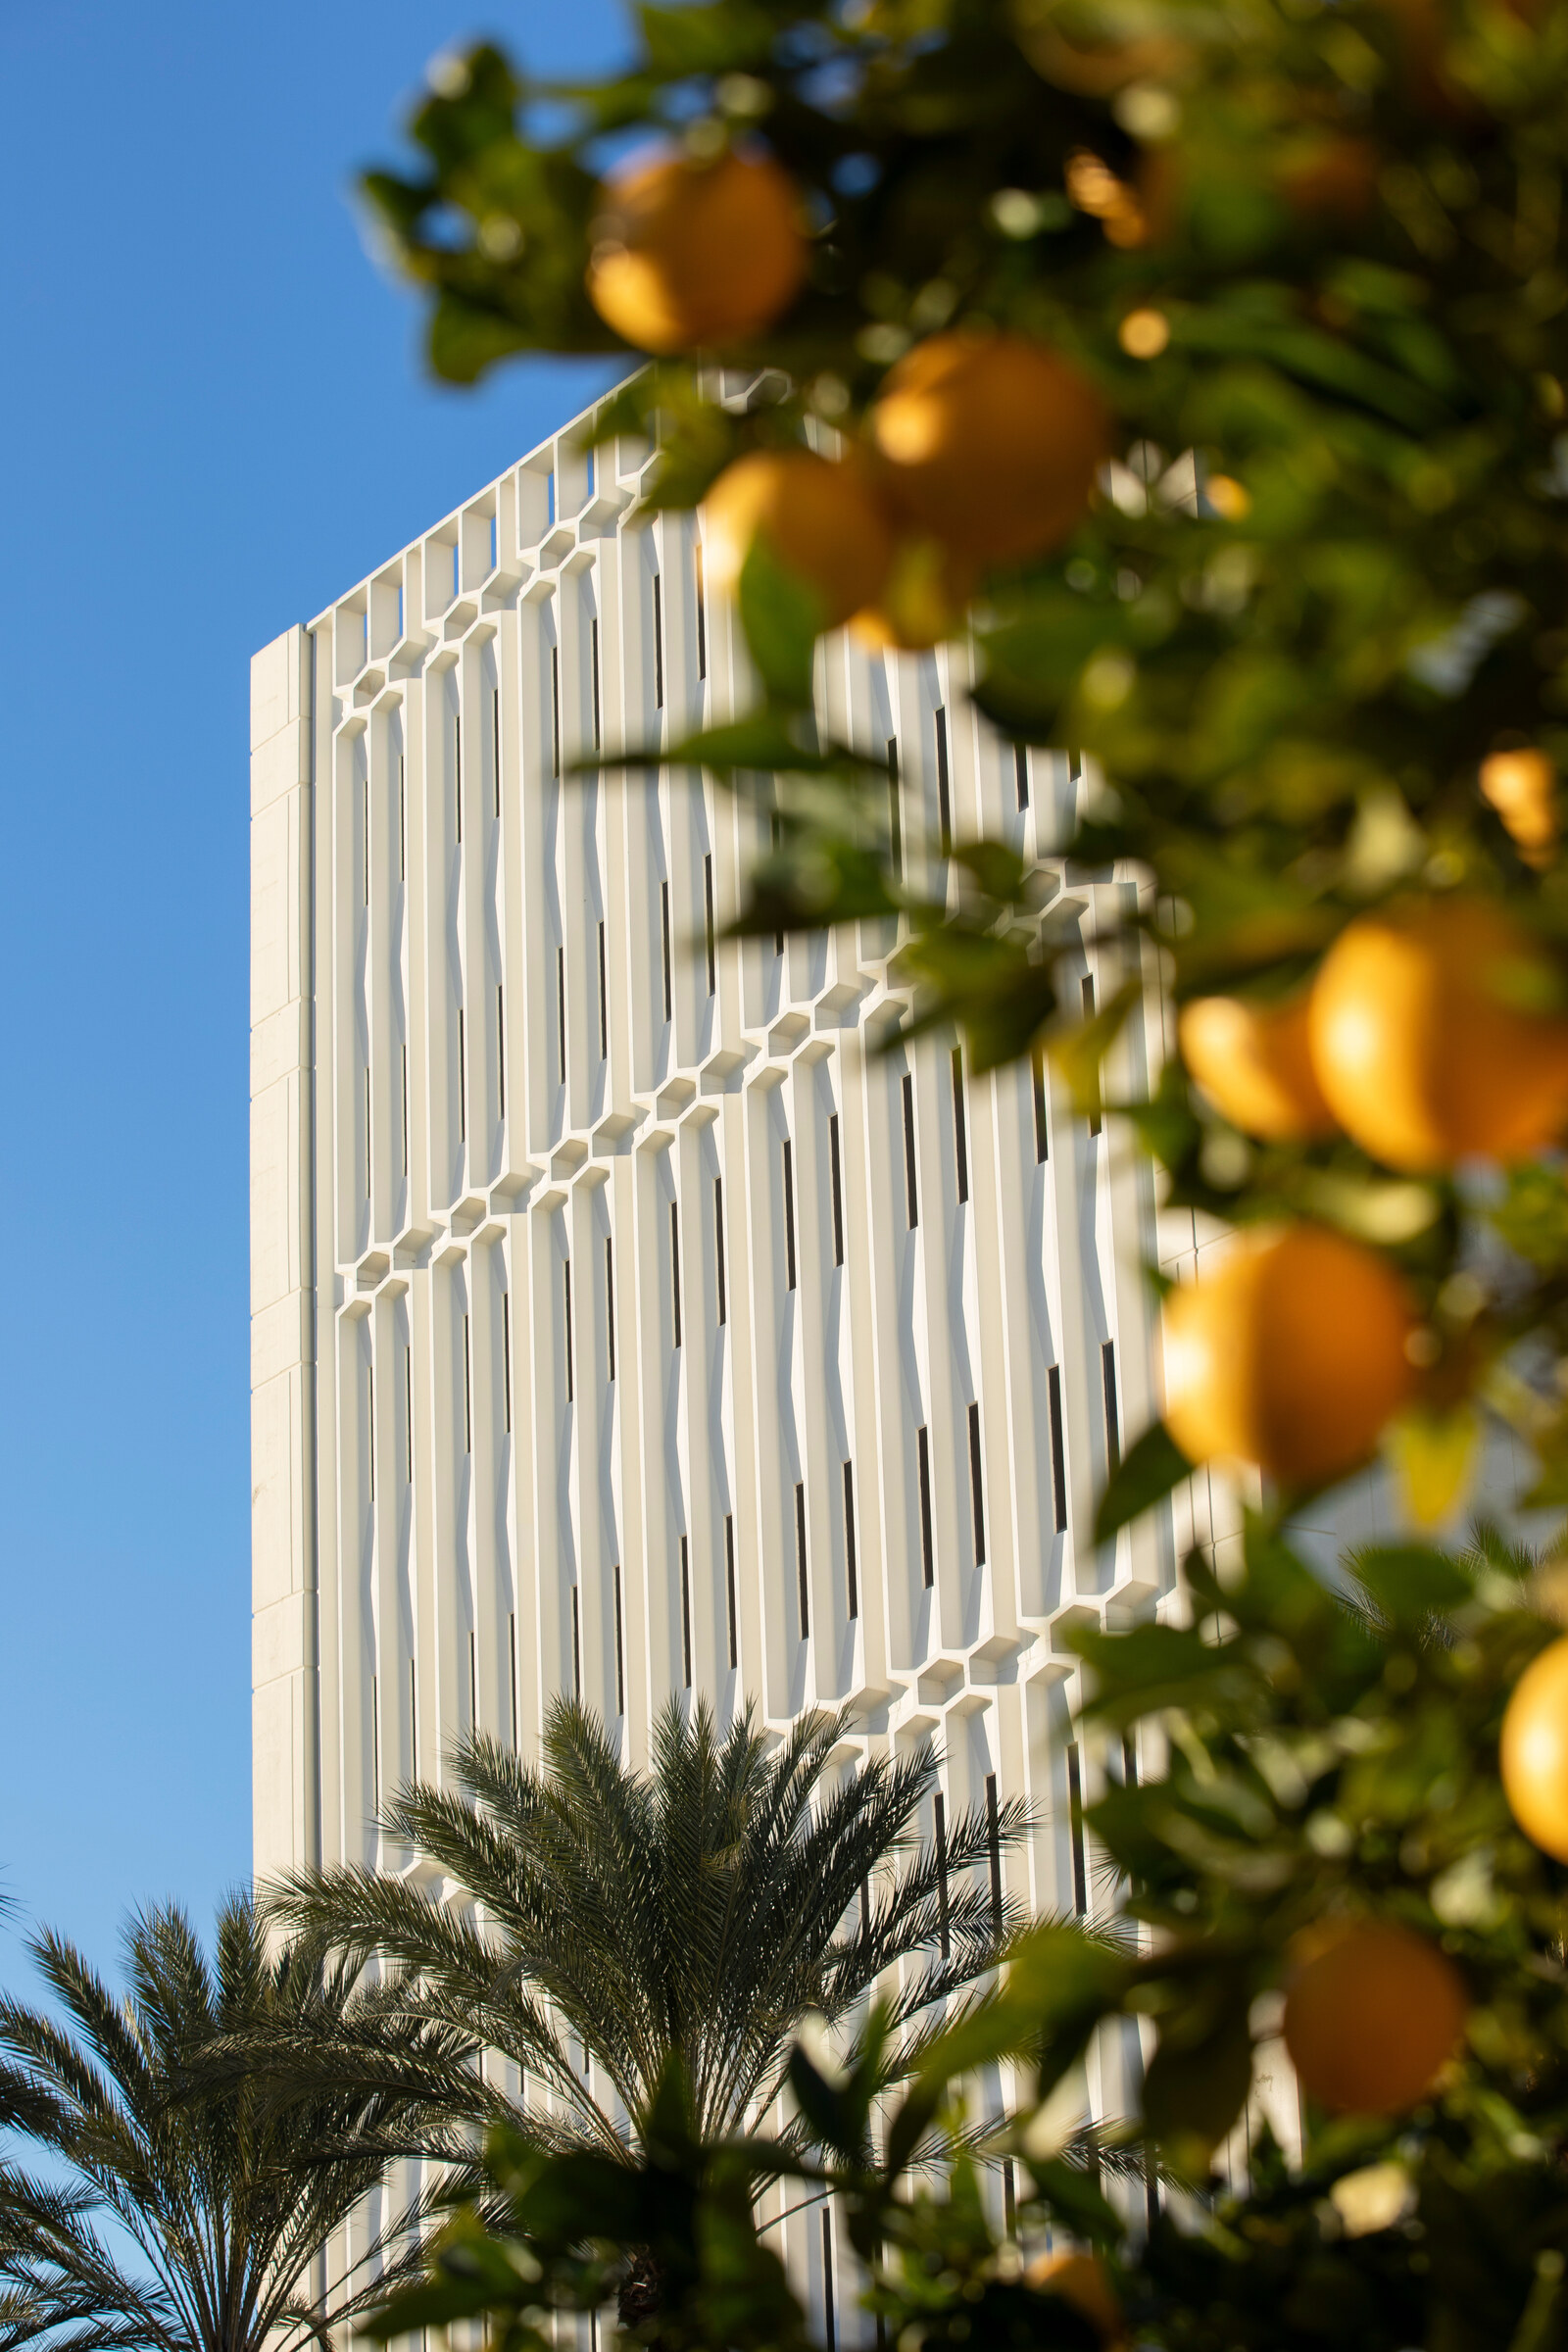
\includegraphics[height=4.6cm,keepaspectratio]{images/campus_orange_tower.jpg}
\end{columns}
\end{frame}

\section{\textcolor{titanorange}{Faculty}}
\begin{frame}{MPA Program Faculty}
\begin{columns}[T,onlytextwidth]
  \column{0.64\textwidth}
  \textbf{Core Faculty}
  \begin{itemize}
    \item Nine full-time faculty members
    \item Diverse research and strong professional experience
    \item Active in scholarship and community engagement
  \end{itemize}
  \column{0.36\textwidth}
  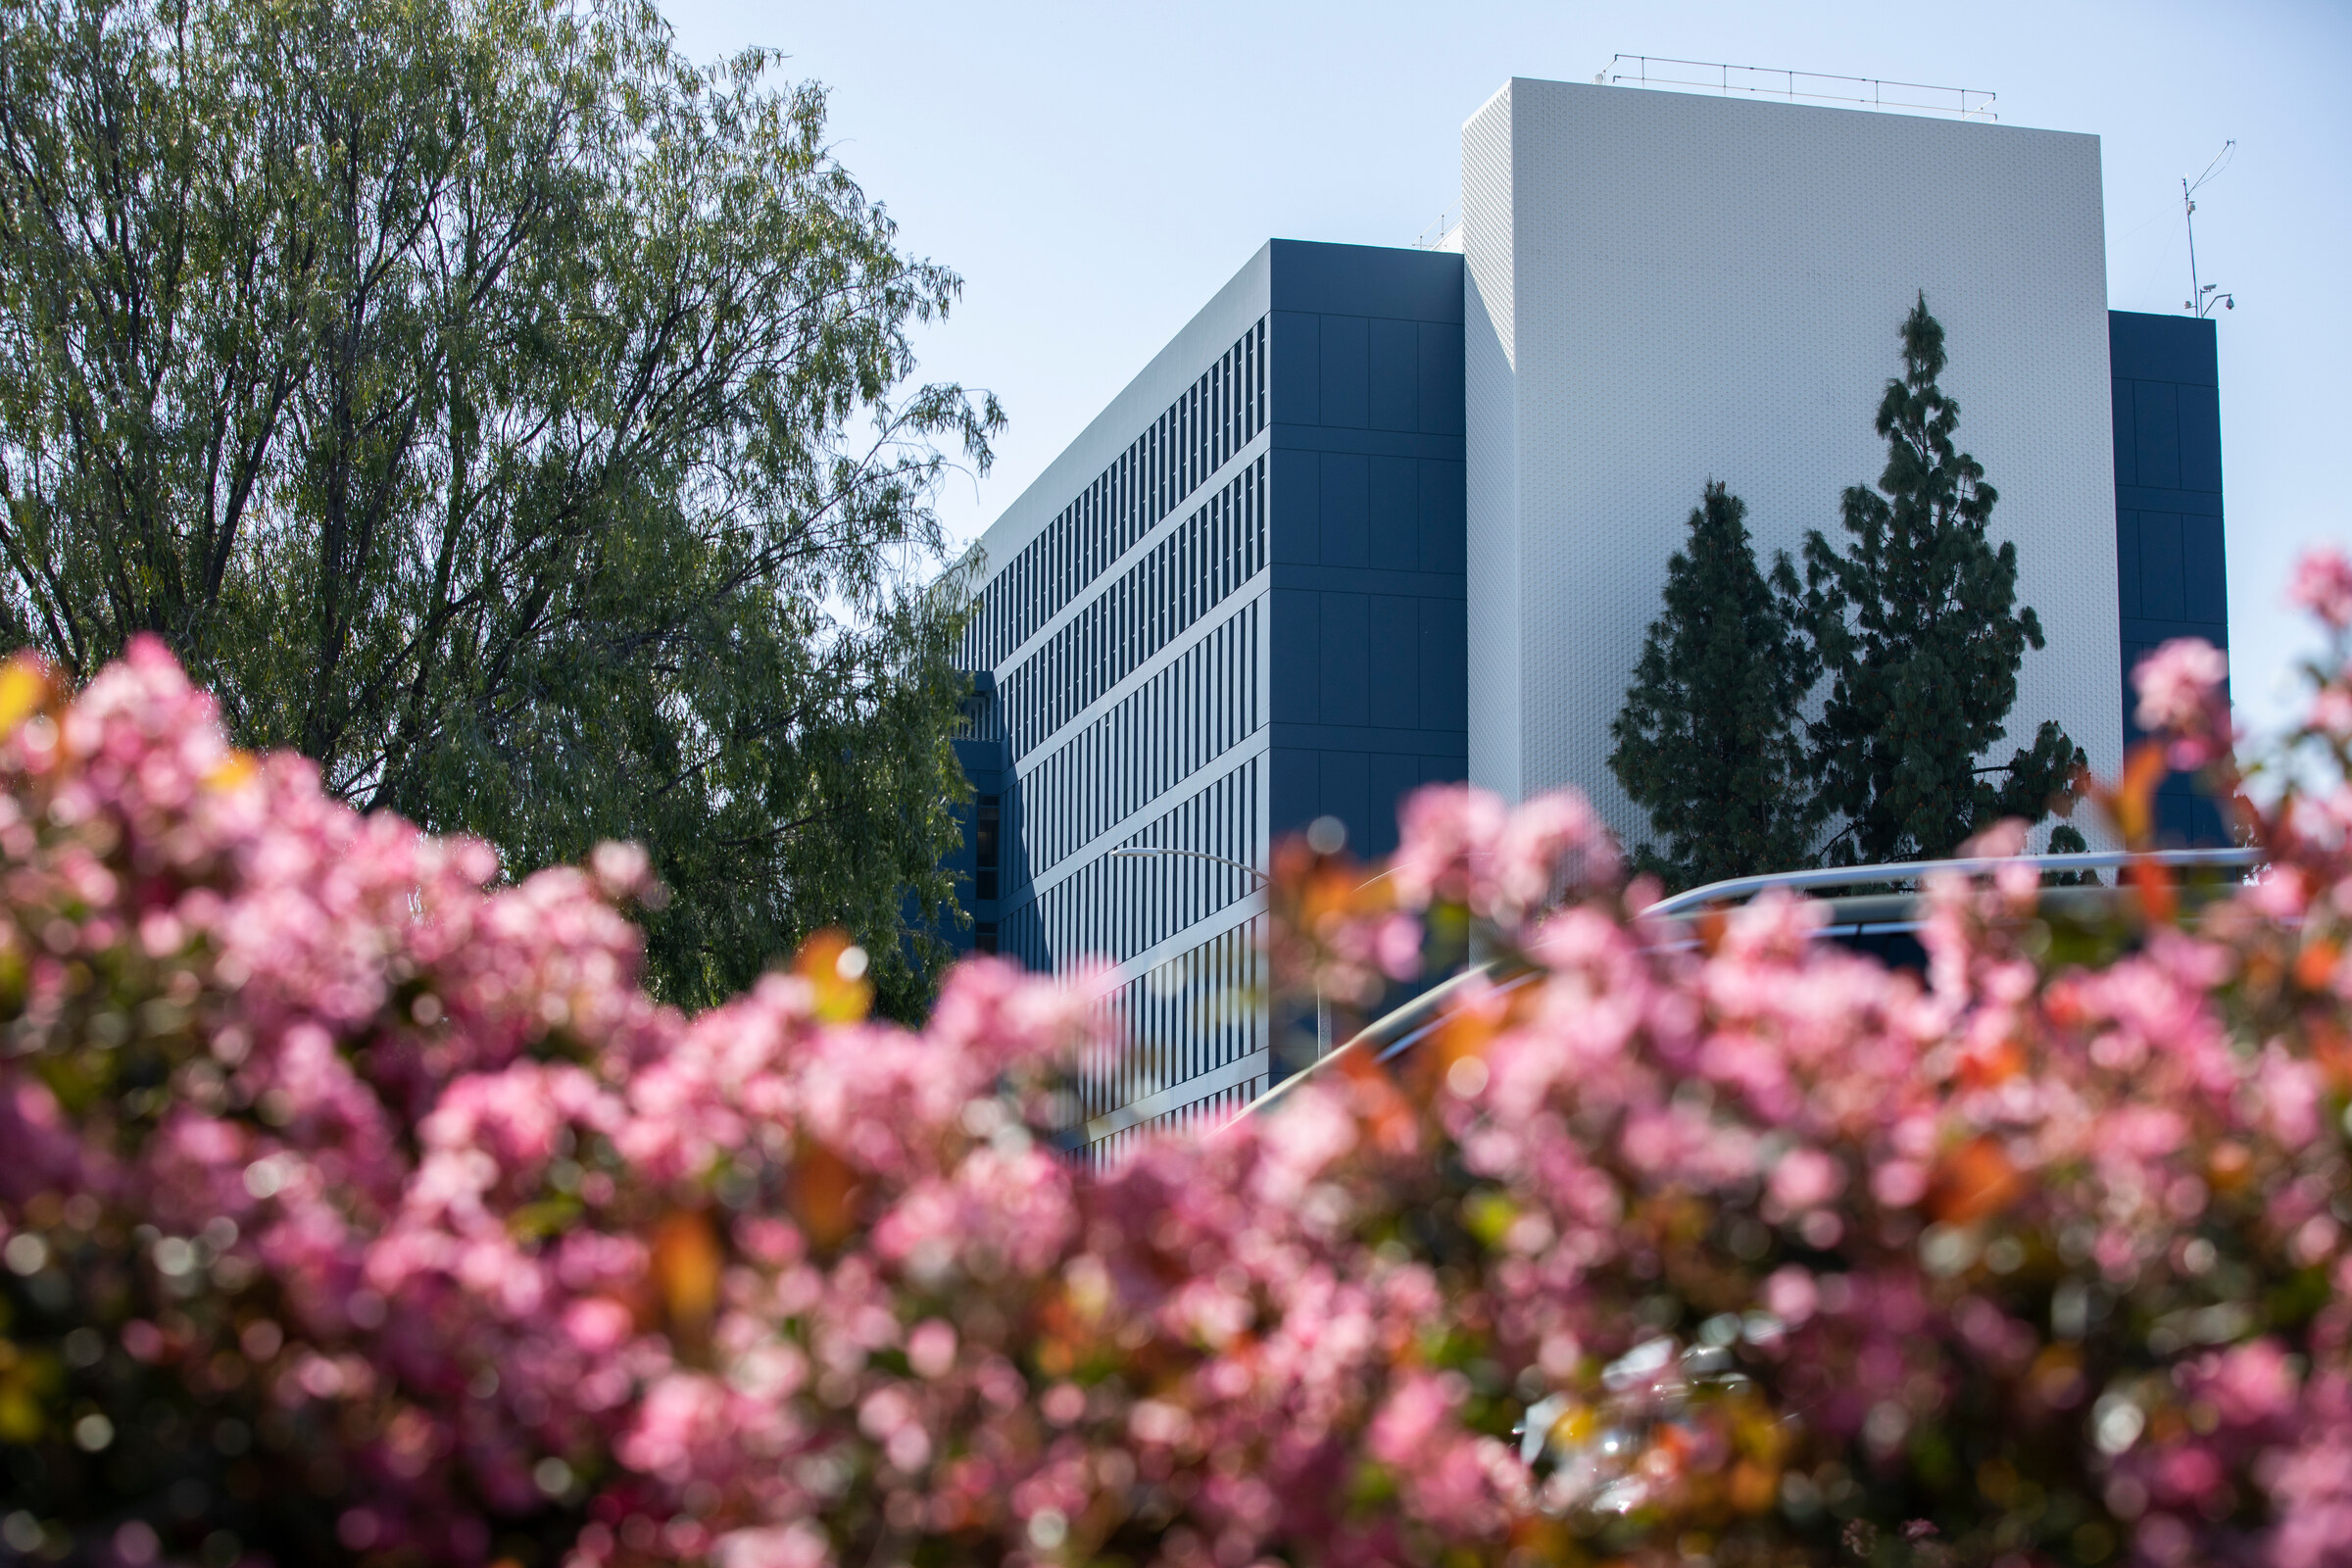
\includegraphics[width=\linewidth]{images/campus_humanities_blossoms.jpg}
\end{columns}
\end{frame}

% Faculty profiles using individual frames instead of problematic macro
\begin{frame}{David P. Adams, Ph.D.}
\begin{columns}[T,onlytextwidth]
  \column{0.66\textwidth}
    \raggedright
    \small
    {\large\bfseries David P. Adams, Ph.D.}\par
    {Associate Professor \& MPA Director}\par
    {\footnotesize At CSUF since 2016 \quad | \quad Ph.D., Auburn University}\par\vspace{0.4em}

    \textbf{Research}
    \begin{itemize}
      \item Environmental Governance
      \item Collaborative Policy
      \item Public Institutions
      \item Technology in Governance
    \end{itemize}

    \textbf{Courses}
    \begin{itemize}
      \item Foundations of PA
      \item Capstone Seminar
      \item Collaborative Governance
    \end{itemize}

  \column{0.34\textwidth}
    \vspace*{0.25cm}
    \FacultyImage{images/adams.jpeg}
\end{columns}
\end{frame}

\begin{frame}{Shelly Arsneault, Ph.D.}
\begin{columns}[T,onlytextwidth]
  \column{0.66\textwidth}
    \raggedright
    {\large\bfseries Shelly Arsneault, Ph.D.}\par
    {Professor}\par
    {\footnotesize At CSUF since 2002 \quad | \quad Ph.D., Michigan State University}\par\vspace{0.4em}

    \textbf{Research}
    \begin{itemize}
      \item Nonprofit management
      \item Education policy
    \end{itemize}

    \textbf{Courses}
    \begin{itemize}
      \item Foundations of PA
      \item Nonprofit Management
      \item Education Policy
    \end{itemize}

  \column{0.34\textwidth}
    \vspace*{0.25cm}
    \FacultyImage{images/arsneault.png}
\end{columns}
\end{frame}

\begin{frame}{Sean Angst, Ph.D.}
\begin{columns}[T,onlytextwidth]
  \column{0.66\textwidth}
    \raggedright
    {\large\bfseries Sean Angst, Ph.D.}\par
    {Assistant Professor}\par
    {\footnotesize At CSUF since 2024 \quad | \quad Ph.D., USC Price}\par\vspace{0.4em}

    \textbf{Research}
    \begin{itemize}
      \item Housing policy
      \item Community development
      \item Racial justice
    \end{itemize}

    \textbf{Courses}
    \begin{itemize}
      \item Administrative Research \& Analysis
      \item Policy Analysis
    \end{itemize}

  \column{0.34\textwidth}
    \vspace*{0.25cm}
    \FacultyImage{images/angst.jpg}
\end{columns}
\end{frame}

\begin{frame}{Clement Mensah Damoah, Ph.D.}
\begin{columns}[T,onlytextwidth]
  \column{0.66\textwidth}
    \raggedright
    {\large\bfseries Clement Mensah Damoah, Ph.D.}\par
    {Assistant Professor}\par
    {\footnotesize At CSUF since 2026 \quad | \quad Ph.D., Arizona State University}\par\vspace{0.4em}

    \textbf{Research}
    \begin{itemize}
      \item Disability and digital inequality
      \item Employment and telework
      \item Socio-digital inclusion
    \end{itemize}

    \textbf{Courses}
    \begin{itemize}
      \item Human Resources Management
      \item Leadership
    \end{itemize}

  \column{0.34\textwidth}
    \vspace*{0.25cm}
    \FacultyImage{images/damoah.jpg}
\end{columns}
\end{frame}

\begin{frame}{Meriem Doucette, Ph.D.}
\begin{columns}[T,onlytextwidth]
  \column{0.66\textwidth}
    \raggedright
    {\large\bfseries Meriem Doucette, Ph.D.}\par
    {Associate Professor}\par
    {\footnotesize At CSUF since 2015 \quad | \quad Ph.D., University of Georgia}\par\vspace{0.4em}

    \textbf{Research}
    \begin{itemize}
      \item Organizational theory
      \item Change management
    \end{itemize}

    \textbf{Courses}
    \begin{itemize}
      \item Organizational Theory
      \item Ethics
      \item Organizational Development
      \item Leadership
    \end{itemize}

  \column{0.34\textwidth}
    \vspace*{0.25cm}
    \FacultyImage{images/doucette.png}
\end{columns}
\end{frame}

\begin{frame}{Elaine Frey, Ph.D.}
\begin{columns}[T,onlytextwidth]
  \column{0.66\textwidth}
    \raggedright
    {\large\bfseries Elaine Frey, Ph.D.}\par
    {Professor}\par
    {\footnotesize Ph.D., George Washington University}\par\vspace{0.4em}

    \textbf{Research}
    \begin{itemize}
      \item Environmental economics
      \item Energy economics
      \item Applied microeconomics
    \end{itemize}

    \textbf{Courses}
    \begin{itemize}
      \item Environmental Policy
      \item Administrative Research \& Analysis
    \end{itemize}

  \column{0.34\textwidth}
    \vspace*{0.25cm}
    \FacultyImage{images/frey.jpg}
\end{columns}
\end{frame}

\begin{frame}{Sarah A. Hill, Ph.D.}
\begin{columns}[T,onlytextwidth]
  \column{0.66\textwidth}
    \raggedright
    {\large\bfseries Sarah A. Hill, Ph.D.}\par
    {Professor \& PAJ Chair}\par
    {\footnotesize At CSUF since 2007 \quad | \quad Ph.D., Caltech}\par\vspace{0.4em}

    \textbf{Research}
    \begin{itemize}
      \item Elections administration
      \item Education policy
    \end{itemize}

    \textbf{Courses}
    \begin{itemize}
      \item State \& Local Government
      \item Public Policy
      \item Diversity in Public Management
    \end{itemize}

  \column{0.34\textwidth}
    \vspace*{0.25cm}
    \FacultyImage{images/hill.jpg}
\end{columns}
\end{frame}

\begin{frame}{Myung--Jung ``MJ'' Kwon, Ph.D.}
\begin{columns}[T,onlytextwidth]
  \column{0.66\textwidth}
    \raggedright
  {\large\bfseries Myung--Jung ``MJ'' Kwon, Ph.D.}\par
    {Professor \& MPA Advisor}\par
    {\footnotesize At CSUF since 2009 \quad | \quad Ph.D., Florida State University}\par\vspace{0.4em}

    \textbf{Research}
    \begin{itemize}
      \item Public sector innovation
      \item E-government
    \end{itemize}

    \textbf{Courses}
    \begin{itemize}
      \item Human Resources Management
      \item Public Personnel Administration
      \item Diversity in Public Management
    \end{itemize}

  \column{0.34\textwidth}
    \vspace*{0.25cm}
    \FacultyImage{images/kwon.jpg}
\end{columns}
\end{frame}

\begin{frame}{Samuel B. Stone, Ph.D.}
\begin{columns}[T,onlytextwidth]
  \column{0.66\textwidth}
    \raggedright
    {\large\bfseries Samuel B. Stone, Ph.D.}\par
    {Professor}\par
    {\footnotesize At CSUF since 2011 \quad | \quad Ph.D., Indiana University}\par\vspace{0.4em}

    \textbf{Research}
    \begin{itemize}
      \item Financial analysis
      \item Fiscal policy
      \item Local government management
    \end{itemize}

    \textbf{Courses}
    \begin{itemize}
      \item Public Finance
      \item Public Budgeting
      \item Local Government Management
    \end{itemize}

  \column{0.34\textwidth}
    \vspace*{0.25cm}
    \FacultyImage{images/stone.jpg}
\end{columns}
\end{frame}

\begin{frame}{Scott Spitzer, Ph.D.}
\begin{columns}[T,onlytextwidth]
  \column{0.66\textwidth}
    \raggedright
    {\large\bfseries Scott Spitzer, Ph.D.}\par
    {Affiliated Faculty \& Professor}\par
    {\footnotesize At CSUF since 2006 \quad | \quad Ph.D., Columbia University}\par\vspace{0.4em}

    \textbf{Research}
    \begin{itemize}
      \item Urban politics
      \item Racial politics
      \item Social welfare
    \end{itemize}

    \textbf{Courses}
    \begin{itemize}
      \item Urban Politics
      \item Metropolitan Politics \& Policy
    \end{itemize}

  \column{0.34\textwidth}
    \vspace*{0.25cm}
    \FacultyImage{images/spitzer.png}
\end{columns}
\end{frame}

\section{\textcolor{titanorange}{Curriculum}}

\begin{frame}{Program Structure}
\begin{Large}
\begin{itemize}
  \item \textbf{Total Units: 36} (12 courses)
  \item Prerequisites
  \item Core courses
  \item One concentration
  \item Electives
  \item Internship (required if no public sector experience)
  \item Comprehensive Exam (embedded in Capstone)
\end{itemize}
\end{Large}
\end{frame}

\begin{frame}{Concentrations}
\begin{Large}
Choose one concentration:
\begin{itemize}
  \item Human Resource Management
  \item Local Government Management
  \item Public Finance
  \item Public Policy
\end{itemize}
\emph{Tip:} Choose a concentration that complements your role and goals.
\end{Large}
\end{frame}

\section{\textcolor{titanorange}{Milestones}}
\begin{frame}{Program Milestones Overview}
\begin{Large}
\centering
\textbf{Your Path to Success}\\[4pt]
\small This timeline represents typical progression. Your path may vary; meet with the MPA advisor to build your sequence.
\end{Large}
\end{frame}

\begin{frame}{Program Orientation}
\begin{Large}
\textbf{Prior to First Semester}
\begin{itemize}
  \item Attend orientation
  \item Review student handbook \small(\url{https://csuf-mpa.github.io/mpa_handbook/})
  \item Complete required paperwork
\end{itemize}
\textbf{Resources}
\begin{itemize}
  \item Academic calendar \small(\url{https://apps.fullerton.edu/AcademicCalendar/})
  \item Campus map \small(\url{https://www.fullerton.edu/campusmap/})
\end{itemize}
\end{Large}
\end{frame}

\begin{frame}{Fall 2026 Key Dates}
\small
\begin{columns}[T,onlytextwidth]
  \column{0.48\textwidth}
  \textbf{Starting the Semester}
  \begin{itemize}\setlength{\itemsep}{4pt}
    \item \textbf{Aug. 17 (Mon):} Academic year begins
    \item \textbf{Aug. 22 (Sat):} First day of classes
    \item \textbf{Sept. 7 (Mon):} Labor Day; campus closed
  \end{itemize}

  \column{0.52\textwidth}
  \textbf{Completing the Semester}
  \begin{itemize}\setlength{\itemsep}{3pt}
    \item \textbf{Nov. 11 (Wed):} Veterans Day; campus closed
    \item \textbf{Nov. 23--29:} Fall Recess; no classes\\
      \footnotesize Campus open Nov. 23--25; closed Nov. 26--27
    \item \textbf{Dec. 11 (Fri):} Last day of classes
    \item \textbf{Dec. 12--18:} Semester examinations
    \item \textbf{Dec. 18 (Fri):} Semester ends
    \item \textbf{Jan. 4, 2027 (Mon):} Grades due
  \end{itemize}
\end{columns}
\end{frame}

\begin{frame}{First Semester Foundations}
\begin{large}
\textbf{Semester One}
\begin{itemize}
  \item Complete POSC 509: Foundations of Public Administration
  \item Take one additional core
  \item \alert{Important:} Take POSC 509 in your first semester.
  \item \alert{Tip:} Use this semester to build foundational knowledge and skills.
  \item \alert{Recommendation:} Join PASA, the Public Administration Student Association.
\end{itemize}
\end{large}
\end{frame}

\begin{frame}{Program Planning}
\begin{Large}
\textbf{Semester Two}
\begin{itemize}
  \item Meet with the MPA advisor
  \item Declare concentration
  \item Complete two core courses
  \item Map your timeline to completion
\end{itemize}
\end{Large}
\end{frame}

\begin{frame}{Mid-Program Achievement}
\begin{Large}
\textbf{At 18 Units}
\begin{itemize}
  \item Maintain 3.0+ GPA
  \item Consider \emph{Pi Alpha Alpha} (3.7+ GPA)
  \item Progress review with advisor
\end{itemize}
\end{Large}
\end{frame}

\begin{frame}{Advanced Phases}
\begin{large}
\textbf{Years 2--3}
\begin{itemize}
  \item Finish three concentration courses
  \item Complete remaining core
\end{itemize}
\textbf{Capstone Prep (Penultimate Semester)}
\begin{itemize}
  \item Complete all core and concentration courses
  \item Be within your final six graduate units
  \item Enroll in POSC 521 (Capstone) for your final semester
  \item Begin comprehensive exam prep
\end{itemize}
\end{large}
\end{frame}

\begin{frame}{Final Steps}
\begin{Large}
\textbf{Final Semester}
\begin{itemize}
  \item File graduation check
    \begin{itemize}
      \item Spring deadline: early February
      \item Fall deadline: early September
    \end{itemize}
  \item Complete Capstone and comprehensive exam
  \item Submit required documentation
  \item Register for commencement
\end{itemize}
\end{Large}
\end{frame}

\section{\textcolor{titanorange}{Scholarships \& Awards}}
\begin{frame}{Scholarships \& Awards}
\large
\begin{itemize}
  \item Lawson Internship in Public Service Award
    \begin{itemize}
      \item \$2{,}000 for a public or nonprofit internship
      \item Apply once enrolled in POSC 497
    \end{itemize}
  \item Alan Saltzstein Excellence Award
    \begin{itemize}
      \item \$1{,}000; typically after completing 6--12 units
      \item Recognizes excellent academic performance
    \end{itemize}
  \item MPA Alumni Scholarship
    \begin{itemize}
      \item \$1{,}000 for first-semester students taking at least two courses
      \item Considers financial need and interest in public service
    \end{itemize}
\end{itemize}
\vspace{0.3em}
\footnotesize Current details and application instructions:
\href{https://paj.fullerton.edu/publicadministration/students/pascholarships.html}{paj.fullerton.edu/publicadministration/students/pascholarships.html}
\end{frame}

\begin{frame}{Graduation Awards}
\large
\begin{itemize}
  \item Sidney Baldwin Award
    \begin{itemize}
      \item Outstanding graduating MPA student; academic achievement and program contribution
    \end{itemize}
  \item Spirit of Public Service Award
    \begin{itemize}
      \item Recognizes a graduating MPA student's public service and involvement
    \end{itemize}
  \item Irving Stone Best Paper Award
    \begin{itemize}
      \item Outstanding public administration course essay from the prior year
    \end{itemize}
\end{itemize}
\end{frame}

\section{\textcolor{titanorange}{Success \& Support}}
\begin{frame}{Keys to Graduate School Success}
\begin{columns}[T,onlytextwidth]
  \column{0.5\textwidth}
  \textbf{Academic}
  \begin{itemize}
    \item Start assignments early
    \item Study groups
    \item Keep detailed cross-course notes
    \item Use office hours
    \item Protect work--life--school balance
  \end{itemize}
  \column{0.5\textwidth}
  \textbf{Professional}
  \begin{itemize}
    \item Network with classmates
    \item Join associations
    \item Consider Pi Alpha Alpha (3.7+)
    \item Build faculty relationships
    \item Start career planning now
  \end{itemize}
\end{columns}

\vspace{0.4em}
\textbf{Time Management}
\begin{itemize}
  \item Plan \(\approx\) 3 hours of study per course hour
  \item Track deadlines
  \item Break big projects into small, dated tasks
\end{itemize}
\end{frame}

{\CSUFUseDarkFooter
\begin{frame}[standout]{Breakout Wrap-Up}
  \huge Questions before we rejoin?
\end{frame}}

\begin{frame}{Start Here: MPA Links}
\centering
\begin{columns}[T,onlytextwidth]
  \column{0.32\textwidth}
    \centering
    \textbf{MPA Home}\\[6pt]
    \qrcode[height=2.15cm]{https://mpa.fullerton.edu}\\[6pt]
    \scriptsize\href{https://mpa.fullerton.edu}{mpa.fullerton.edu}

  \column{0.36\textwidth}
    \centering
    \textbf{Student Handbook}\\[6pt]
    \qrcode[height=2.15cm]{https://csuf-mpa.github.io/mpa_handbook/}\\[6pt]
    \scriptsize\href{https://csuf-mpa.github.io/mpa_handbook/}{csuf-mpa.github.io/mpa\_handbook}

  \column{0.32\textwidth}
    \centering
    \textbf{Join PASA}\\[6pt]
    \qrcode[height=2.15cm]{https://fullerton.campuslabs.com/engage/organization/pasa}\\[6pt]
    \scriptsize\href{https://fullerton.campuslabs.com/engage/organization/pasa}{PASA on TitanLink}
\end{columns}
\end{frame}

\section{\textcolor{titanorange}{Campus Resources}}

\begin{frame}{Campus Resources: Academic \& Graduate Support}
\begin{columns}[T,onlytextwidth]
  \column{0.5\textwidth}
  \begin{block}{Academic Support}
    \begin{itemize}\setlength{\itemsep}{4pt}
      \item \textbf{Pollak Library}\\[-2pt]
        \footnotesize\href{https://library.fullerton.edu}{library.fullerton.edu}
      \item \textbf{Computer Labs}\\[-2pt]
        \footnotesize\href{https://www.fullerton.edu/it/services/computer-labs/}{fullerton.edu/it/services/computer-labs}
    \end{itemize}
  \end{block}

  \column{0.5\textwidth}
  \begin{block}{Graduate Support}
    \begin{itemize}\setlength{\itemsep}{4pt}
      \item \textbf{Graduate Studies}\\[-2pt]
        \footnotesize\href{https://www.fullerton.edu/graduate}{fullerton.edu/graduate}
      \item \textbf{Graduate Studies Center (GSC)}\\[-2pt]
        \footnotesize\href{https://www.fullerton.edu/graduate/gsc/index.html}{fullerton.edu/graduate/gsc}
    \end{itemize}
  \end{block}
\end{columns}
\end{frame}

\begin{frame}{Student Services}
\begin{columns}[T,onlytextwidth]
  \column{0.5\textwidth}
  \begin{block}{ID, Campus Access, \& Logistics}
    \begin{itemize}\setlength{\itemsep}{4pt}
      \item \textbf{TitanCard}\\[-2pt]
        \footnotesize\href{https://www.fullerton.edu/it/services/titancard/}{fullerton.edu/it/services/titancard}
      \item \textbf{Parking \& Transportation}\\[-2pt]
        \footnotesize\href{https://parking.fullerton.edu}{parking.fullerton.edu}
      \item \textbf{Titan Shops}\\[-2pt]
        \footnotesize\href{https://www.titanbookstore.com}{titanbookstore.com}
    \end{itemize}
  \end{block}

  \column{0.5\textwidth}
  \begin{block}{Money, Records, \& Enrollment}
    \begin{itemize}\setlength{\itemsep}{4pt}
      \item \textbf{Financial Aid}\\[-2pt]
        \footnotesize\href{https://www.fullerton.edu/financialaid}{fullerton.edu/financialaid}
      \item \textbf{Registrar}\\[-2pt]
        \footnotesize\href{https://registrar.fullerton.edu/}{registrar.fullerton.edu}
      \item \textbf{Student Wellness}\\[-2pt]
        \footnotesize\href{https://www.fullerton.edu/studentwellness}{fullerton.edu/studentwellness}
    \end{itemize}
  \end{block}
\end{columns}
\end{frame}

\begin{frame}{Support Services \& Resource Centers}
\footnotesize
\begin{columns}[T,onlytextwidth]
  \column{0.42\textwidth}
  \begin{block}{Student Support}
    \begin{itemize}\setlength{\itemsep}{2pt}
      \item \textbf{Career Center}\\[-2pt]
        {\scriptsize\href{https://www.fullerton.edu/career}{fullerton.edu/career}}
      \item \textbf{Disability Support Services}\\[-2pt]
        {\scriptsize\href{https://www.fullerton.edu/dss/}{fullerton.edu/dss}}
      \item \textbf{Veterans Resource Center}\\[-2pt]
        {\scriptsize\href{https://www.fullerton.edu/veterans}{fullerton.edu/veterans}}
    \end{itemize}
  \end{block}

  \column{0.58\textwidth}
  \begin{block}{Identity-Based Resource Centers}
    \begin{itemize}\setlength{\itemsep}{2pt}
      \item \textbf{Women's Resource Center}\\[-2pt]
        {\scriptsize\href{https://www.fullerton.edu/wrc/}{fullerton.edu/wrc}}
      \item \textbf{Titan Dreamers Resource Center}\\[-2pt]
        {\scriptsize\href{https://www.fullerton.edu/tdrc/}{fullerton.edu/tdrc}}
      \item \textbf{Asian Pacific American Resource Center}\\[-2pt]
        {\scriptsize\href{https://www.fullerton.edu/aparc/}{fullerton.edu/aparc}}
      \item \textbf{Native American \& Indigenous Resource Center}\\[-2pt]
        {\scriptsize\href{https://www.fullerton.edu/nairc/}{fullerton.edu/nairc}}
      \item \textbf{Losquadro Keller LGBTQ+ Resource Center}\\[-2pt]
        {\scriptsize\href{https://www.fullerton.edu/lgbtq/}{fullerton.edu/lgbtq}}
    \end{itemize}
  \end{block}
\end{columns}
\end{frame}

\begin{frame}{Additional Support Resources}
\begin{columns}[T,onlytextwidth]
  \column{0.52\textwidth}
  \begin{block}{Basic Needs}
    \begin{itemize}\setlength{\itemsep}{4pt}
      \item \textbf{Tuffy's Basic Needs}\\[-2pt]
        \footnotesize\href{https://www.fullerton.edu/basic-needs/}{fullerton.edu/basic-needs}
      \item \textbf{ASI Food Pantry \& Food Resources}\\[-2pt]
        \footnotesize\href{https://www.fullerton.edu/basic-needs/calfresh/food.html}{fullerton.edu/basic-needs/calfresh/food}
    \end{itemize}
  \end{block}

  \column{0.48\textwidth}
  \begin{block}{Family Support}
    \begin{itemize}\setlength{\itemsep}{4pt}
      \item \textbf{Children's Center}\\[-2pt]
        \footnotesize\href{https://asi.fullerton.edu/childrens-center}{asi.fullerton.edu/childrens-center}
    \end{itemize}
  \end{block}
\end{columns}
\end{frame}

\begin{frame}{Your Next Five Actions}
\large
\begin{enumerate}\setlength{\itemsep}{7pt}
  \item Confirm your Fall schedule includes \textbf{POSC 509} and one additional core course.
  \item Bookmark \href{https://mpa.fullerton.edu}{\textbf{mpa.fullerton.edu}} and the \href{https://csuf-mpa.github.io/mpa_handbook/}{\textbf{MPA Student Handbook}}.
  \item Check CSUF email, Canvas, and Titan Online; include your CWID when contacting staff.
  \item Join \href{https://fullerton.campuslabs.com/engage/organization/pasa}{\textbf{PASA on TitanLink}}.
  \item Set a second-semester advising reminder and email \href{mailto:mpaadvising@fullerton.edu}{\textbf{mpaadvising@fullerton.edu}}.
\end{enumerate}
\end{frame}

\section{\textcolor{titanorange}{Contact}}
\begin{frame}{Contact Information}
\small
\textbf{MPA Program Office (GH-511; Monday--Friday, 8 a.m.--5 p.m.)}\\[-2pt]
\begin{itemize}
  \item Email: \href{mailto:mpaprogram@fullerton.edu}{mpaprogram@fullerton.edu}
  \item Phone: 657--278--3521
\end{itemize}

\textbf{MPA Advisor -- Myung--Jung ``MJ'' Kwon (GH-523)}\\[-2pt]
\begin{itemize}
  \item Email: \href{mailto:mpaadvising@fullerton.edu}{mpaadvising@fullerton.edu}
  \item Phone: 657--278--2446; email to schedule an appointment
\end{itemize}

\textbf{MPA Director -- David P. Adams (GH-516)}\\[-2pt]
\begin{itemize}
  \item Email: \href{mailto:dpadams@fullerton.edu}{dpadams@fullerton.edu}
  \item Phone: 657--278--7279
  \item Appointments: \url{https://dadams.io/appointments}
\end{itemize}
\end{frame}

{\CSUFUseDarkFooter
\begin{frame}[standout]{Questions?}
  \huge{Large Group Q \& A}
\end{frame}}

\begin{frame}{Thank You for Attending}
\centering

\includegraphics[height=3cm]{images/PUBLIC-ADMINISTRATION-color.png}\\[10pt]
\textbf{Master of Public Administration (MPA) Program}\\
\textbf{New Student Orientation}
\end{frame}

\end{document}
